\reportpage{03 / THE REPRODUCIBLE EXPERIMENT}{How much does a century of motion change access?}
We ask a narrower question than ``how many planets will be found?'': for the \emph{same} nearby-source sample and hypothetical planet population, how does relative motion change single-visit direct-imaging accessibility? Four paired scenarios separate geometry from an assumed improvement in instrument thresholds.
\begin{center}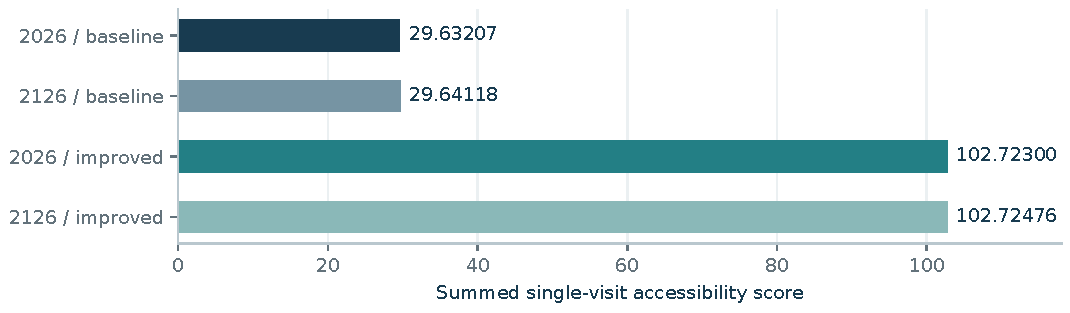
\includegraphics[width=\linewidth,height=55mm,keepaspectratio]{scores.pdf}\end{center}
\figcap{The baseline geometry change is visually tiny beside the chosen instrument change. Bar lengths are sums of conditional accessibility fractions, not planet counts. All four scenarios use the same \ReportSampleSize{} selected Gaia DR3 sources.}

\begin{minipage}[t]{.485\linewidth}\vspace{0pt}\setlength{\parskip}{3pt}
\subsection*{Data and assumptions}
Gaia DR3 selection [4]: parallax $\geq50$ mas, parallax signal-to-noise $>20$, measured radial velocity, RUWE $<1.4$ and at least ten visibility periods. This is not a complete nearby-star census.

Each source receives a hypothetical Earth-radius planet on a circular 1 AU orbit with geometric albedo 0.3. The score averages over isotropic orientations and phases.

\small\begin{tabularx}{\linewidth}{@{}Xrr@{}}\toprule
Threshold & Baseline & Improved\\\midrule
Inner working angle & 60 mas & 40 mas\\
Contrast floor & $10^{-10}$ & $5\!\times\!10^{-11}$\\
Planet magnitude limit & $G=30$ & $G=31$\\\bottomrule
\end{tabularx}\par\vspace{4pt}\normalsize
\end{minipage}\hfill
\begin{minipage}[t]{.485\linewidth}\vspace{0pt}\setlength{\parskip}{3pt}
\subsection*{Result and uncertainty}
The baseline sum changes from \textbf{\ReportBaselineInitial{} to \ReportBaselineFuture{}}. The motion contribution is
\[
 \Delta S_{\mathrm{motion}}=\ReportMotionScore\quad(\ReportMotionPercent\%).
\]
The assumed instrument change adds \textbf{\ReportInstrumentScore{}} at the initial epoch. These settings are sensitivity scenarios, not specifications for an approved telescope.

With \ReportDraws{} correlated astrometric draws per source, the formal 95\% interval for the motion difference is \textbf{\ReportMotionLow{} to \ReportMotionHigh{}}. It excludes population and instrument uncertainty, binary-system errors and cross-source systematics.
\end{minipage}

\subsection*{What the score actually measures}
For isotropic planet positions, $\cos\alpha$ is uniform. If the simultaneous angular-separation, contrast and magnitude conditions admit $[\alpha_{\min},\alpha_{\max}]$, then
\begin{equation}
 C_i=\frac{\cos\alpha_{\min}-\cos\alpha_{\max}}{2},\qquad
 S=\sum_{i=1}^{\ReportSampleSizeMath} C_i,
\end{equation}
with $C_i=0$ for an empty interval. Averaging over orientation removes sensitivity to the absolute sky direction. Thus this experiment tests distance, brightness and separation thresholds; it does \emph{not} follow known orbital planes into new transit bands.

\takeaway{A counterexample to ``waiting helps''}{At the baseline settings, \ReportGainers{} sources gain and \ReportLosers{} lose accessibility. Changing only the inner working angle to 70 mas gives a net motion contribution near \textbf{$\ReportSensitivitySeventy$}. These are changes in scores, not discoveries. The next step is a targeted study with measured planetary orbital geometry.}
